\begin{figure}[H]
    \centering
    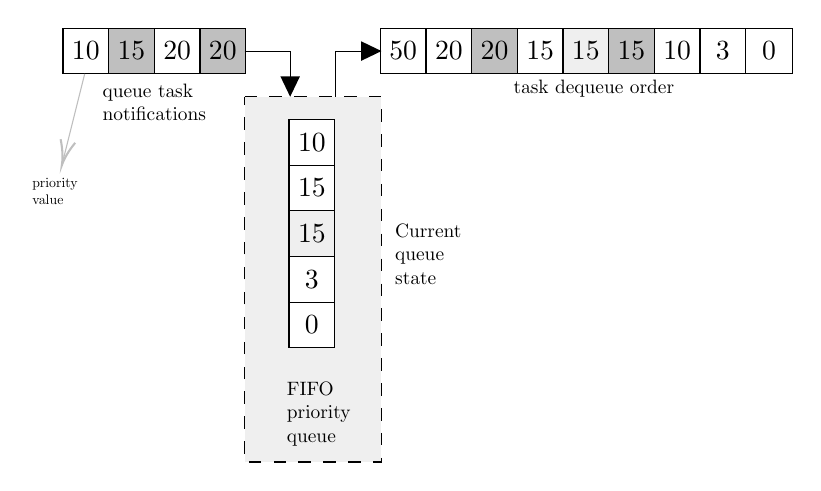
\begin{tikzpicture}[x=0.75pt,y=0.75pt,yscale=-1,xscale=1, scale=1.1]
        \draw   (100.5,50) -- (120.5,50) -- (120.5,70) -- (100.5,70) -- cycle ;
        \draw  [fill=gray!50  ,fill opacity=1 ] (120.5,50) -- (140.5,50) -- (140.5,70) -- (120.5,70) -- cycle ;
        \draw   (140.5,50) -- (160.5,50) -- (160.5,70) -- (140.5,70) -- cycle ;
        \draw  [fill=gray!50  ,fill opacity=1 ] (160.5,50) -- (180.5,50) -- (180.5,70) -- (160.5,70) -- cycle ;
        \draw   (239.5,50) -- (259.5,50) -- (259.5,70) -- (239.5,70) -- cycle ;
        \draw  [fill=white  ,fill opacity=1 ] (259.5,50) -- (279.5,50) -- (279.5,70) -- (259.5,70) -- cycle ;
        \draw   (299.5,50) -- (319.5,50) -- (319.5,70) -- (299.5,70) -- cycle ;
        \draw  [fill=gray!50  ,fill opacity=1 ] (279.5,50) -- (299.5,50) -- (299.5,70) -- (279.5,70) -- cycle ;
        \draw  [color=black  ,draw opacity=1 ][fill=lightgray!25  ,fill opacity=1 ][dash pattern={on 4.5pt off 4.5pt}] (180,80) -- (240,80) -- (240,240) -- (180,240) -- cycle ;
        \draw    (180,60) -- (200,60) -- (200,78) ;
        \draw [shift={(200,80)}, rotate = 270] [fill=black  ][line width=0.75]  [draw opacity=0] (8.93,-4.29) -- (0,0) -- (8.93,4.29) -- cycle;
        \draw  [fill=lightgray!25  ,fill opacity=1 ] (319.5,50) -- (339.5,50) -- (339.5,70) -- (319.5,70) -- cycle ;
        \draw  [fill=gray!50  ,fill opacity=1 ] (339.5,50) -- (359.5,50) -- (359.5,70) -- (339.5,70) -- cycle ;
        \draw   (359.5,50) -- (379.5,50) -- (379.5,70) -- (359.5,70) -- cycle ;
        \draw  [fill=white  ,fill opacity=1 ] (379.5,50) -- (399.5,50) -- (399.5,70) -- (379.5,70) -- cycle ;
        \draw  [fill=white  ,fill opacity=1 ] (399.5,50) -- (420,50) -- (420,70) -- (399.5,70) -- cycle ;
        \draw    (220,80) -- (220,60) -- (238,60) ;
        \draw [shift={(240,60)}, rotate = 180] [fill=black  ][line width=0.75]  [draw opacity=0] (8.93,-4.29) -- (0,0) -- (8.93,4.29) -- cycle;
        \draw [color=gray!50  ,draw opacity=1 ]   (110,70) -- (100.49,108.06) ;
        \draw [shift={(100,110)}, rotate = 284.04] [color=gray!50  ,draw opacity=1 ][line width=0.75]    (10.93,-3.29) .. controls (6.95,-1.4) and (3.31,-0.3) .. (0,0) .. controls (3.31,0.3) and (6.95,1.4) .. (10.93,3.29)   ;
        \draw  [fill=white  ,fill opacity=1 ] (199.5,90) -- (219.5,90) -- (219.5,110) -- (199.5,110) -- cycle ;
        \draw  [fill=white  ,fill opacity=1 ] (199.5,110) -- (219.5,110) -- (219.5,130) -- (199.5,130) -- cycle ;
        \draw  [fill=lightgray!25  ,fill opacity=1 ] (199.5,130) -- (219.5,130) -- (219.5,150) -- (199.5,150) -- cycle ;
        \draw  [fill=white  ,fill opacity=1 ] (199.5,150) -- (219.5,150) -- (219.5,170) -- (199.5,170) -- cycle ;
        \draw  [fill=white  ,fill opacity=1 ] (199.5,170) -- (219.5,170) -- (219.5,190) -- (199.5,190) -- cycle ;
        \draw (110.5,60) node  [align=left] {10};
        \draw (130.5,60) node  [align=left] {15};
        \draw (150.5,60) node  [align=left] {20};
        \draw (170.5,60) node  [align=left] {20};
        \draw (249.5,60) node  [align=left] {50};
        \draw (269.5,60) node  [align=left] {20};
        \draw (289.5,60) node  [align=left] {20};
        \draw (309.5,60) node  [align=left] {15};
        \draw (369.5,60) node  [align=left] {10};
        \draw (329.5,60) node  [align=left] {15};
        \draw (349.5,60) node  [align=left] {15};
        \draw (389.5,60) node  [align=left] {3};
        \draw (409.75,60) node  [align=left] {0};
        \draw (260.5,149) node [scale=0.7] [align=left] {Current\\queue\\state};
        \draw (333,76.5) node [scale=0.7] [align=left] {task dequeue order};
        \draw (140.5,82.5) node [scale=0.7] [align=left] {queue task \\notifications};
        \draw (97,121.5) node [scale=0.5] [align=left] {priority\\value};
        \draw (209.5,100) node  [align=left] {10};
        \draw (209.5,120) node  [align=left] {15};
        \draw (209.5,140) node  [align=left] {15};
        \draw (209.5,160) node  [align=left] {3};
        \draw (209.5,180) node  [align=left] {0};
        \draw (212.5,219) node [scale=0.7] [align=left] {FIFO\\priority\\queue};
    \end{tikzpicture}
    \caption{Priority-queue behavior}
    \label{fig:prioqueue}
\end{figure}